%!TEX root = Constructive Alignment for Introductory Programming.tex

\chapter{Approaches to Constructive Alignment} % (fold)
\label{cha:background}

\cite{DeRaadt:2005} approach to learning  had the strongest correlation to success as compared to other cognitive and demographic measures.

\section{Constructive Alignment} % (fold)
\label{sec:constructive_alignment}

Constructive alignment, as proposed by Biggs~\cite{Biggs:1996c}, is an amalgamation of constructive learning theory and aligned instruction design. It aims to elicit deep learning approaches from all students. Biggs' model is student focused, with clear and intentional alignment of assessment, teaching and learning activities, and unit objectives. The focus on the central role of the learner in building meaning is derived from constructivist learning theories, whilst the alignment of assessment, teaching, and learning activities, has its foundation in instructional design literature. 

\fref{fig:constructive_alignment} illustrates the constructive alignment model presented in~\cite{Houghton:2004}, which consists of the following blocks:

\begin{itemize}
	\item \emph{Intended learning outcomes} clearly define required learning in terms of ``performances of understanding''.
	\item \emph{Performance objectives} emerge from the desired outcomes, and can be ranked to become the assessment criteria.
	\item \emph{Teaching and learning activities} are designed to place students in situations likely to elicit the required learning.
	\item Students provide \emph{evidence of their learning}, that is assessed against the criteria to determine grade outcomes.
\end{itemize}

% \begin{figure}[t!]
% 	\centering
% 	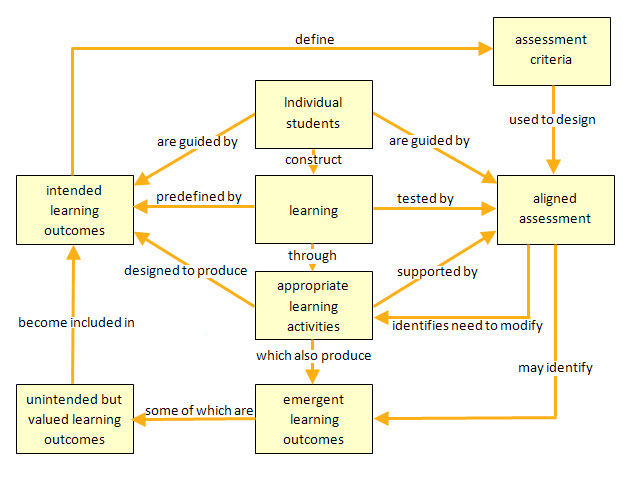
\includegraphics[width=\columnwidth]{Houghton_constructive_alignment_1}
% 	\caption{Constructive alignment model presented by Houghton in~\cite{Houghton:2004}}
% 	\label{fig:constructive_alignment}
% \end{figure}

\subsection{Constructivism} % (fold)
\label{sub:constructivism}

In designing teaching and learning contexts, educators use some form of theory of teaching and learning to guide their decision making.

theory of teaching and learning

espoused theory \cite{Argyris:1976}

\emph{objectivist}

\emph{constructivism} and \emph{phenomenography}


\cite{Duffy:1996} 




\cite{Montessori:1946}

Constructivism is a theory of knowledge that focuses on the active role of the learner in constructing their own understanding. Dating back to \citet{Piaget:1950} constructivism exists in several forms: cognitive, individual, postmodern, radical and social constructivism \cite{Phillips:1995,Steffe:1995}. Each of these forms of constructivism has various implications for teaching and learning.









In his original paper on constructive alignment \citet{Biggs:1996c} adopted constructivism as a framework to help guide decision making in all facets of teaching and learning. Constructivism was chosen over phenomenography 

practical concerns


For this work we are interested in adapting \emph{constructive learning theories}

 taking practical aspects from constructivism in general and focusing on what the student does, as suggested by .


In proposing constructive alignment, 

Disconnect between theory in use and espoused theory: \cite{Phillips:2005}


Engage with and expand experience \cite{Dewey:1960} exploration, thinking and reflection

% subsection constructivism (end)

\subsection{Aligned Curriculum} % (fold)
\label{sub:aligned_curriculum}

% subsection aligned_curriculum (end)

\subsection{Reported Applications of Constructive Alignment} % (fold)
\label{sub:reported_applications_of_constructive_alignment}

% subsection reported_applications_of_constructive_alignment (end)

% section constructive_alignment (end)

\section{Portfolio Assessment} % (fold)
\label{sec:portfolio_assessment}

% section portfolio_assessment (end)




% chapter background (end)